
\section{Machine Learning Pipeline}\label{sec:machine_learning_pipeline}

In this section, we explain the machine learning pipeline that converts vacancy posting text into continuous numerical 
vectors. We leverage the structured nature of job descriptions to extract high-signal information efficiently. Job 
descriptions, despite their length, follow a consistent format. We focus on the easily detectable Mandatory and 
Desired Skills sections, which provide concentrated information about skill and competency requirements. Using the 
Spacy natural language processing library, we parse these sections to extract key technical skills such as programming 
languages (e.g., Java, Asp.Net), web frameworks (e.g., Django), and testing tools (e.g., Selenium).

While knowledge of technologies is important, the Responsibilities section conveys crucial functional aspects of the 
role. These can vary notably even between positions requiring similar technology skills, such as developers, testers, 
and support engineers. The section typically lists tasks to be performed, which might include 'develop big data strategy,' 
'conduct code reviews,' 'engage with stakeholders' or 'application development.' We extract such task descriptions from 
job responsibilities by employing natural language processing techniques. This includes part-of-speech tagging to identify 
action verbs and dependency parsing to locate their direct objects, which are then combined to form concise verb-object 
phrases representing key tasks. By leveraging the structured format and our knowledge of the postings, we effectively 
eliminate low-signal words in the description. In the following subsections, we describe our machine learning pipeline 
which adheres to two key ideas: leveraging capabilities of a pre-trained language model and utilizing past selection 
decisions. 

\subsection{Pre-trained Embeddings}
Here we describe the approach to mapping the extracted text from job postings to the embedding space of 
a pre-trained language model. This section focuses on generating robust embeddings for informativeness 
assessment, rather than achieving state-of-the-art performance on general semantic similarity tasks. 
Prior to embedding, standard pre-processing steps such as lowercasing, stop word removal, and punctuation 
normalization were applied to refine the text.

To create vector representations of the two parts we employ Sentence-BERT (SBERT), a modification of 
the pre-trained BERT network \citep{devlin2018bert}. SBERT is designed to derive semantically meaningful 
sentence embeddings, making it more efficient for comparing longer text strings than BERT embeddings, which 
are typically word vectors, although the BERT word-level embeddings vary with the context, unlike their 
predecessors \citep{reimers-2019-sentence-bert}. SBERT converts text into dense vector representations, 
effectively capturing the semantic meanings and relationships between words. This model is particularly 
suitable for our needs because it is pre-trained and fine-tuned for similarity tasks, ensuring that it 
can generate fixed-size embeddings that are both informative and consistent. The embeddings are generated 
using the SentenceTransformers library (model: paraphrase-MiniLM-L6-v2). By leveraging SBERT, we ensure that 
our embeddings capture the nuanced language used in job postings, which is critical for accurately representing 
the skills and tasks.

For every job posting $j_i$, we have the set of words $j_i^s$ (skills) and $j_i^t$ (tasks) and obtain SBERT 
embeddings $e_i^s$ ($384 \times 1$) and $e_i^t$ ($384 \times 1$) respectively. This separation allows for 
more granular embeddings and a focused semantic representation of each aspect. To evaluate the benefit of 
this separation, we also conducted a baseline experiment where the 'Mandatory Skills,' 'Desired Skills,' 
and 'Responsibilities' sections were concatenated before embedding (referred to as the 'no-split' approach). 
These embeddings encapsulate the semantic content of the job postings, allowing us to compare and analyze 
them effectively. The dual-embedding approach provides a comprehensive view of each position, highlighting 
both the required competencies and the associated responsibilities. This detailed representation forms the 
foundation for developing a robust distance metric that can accurately reflect the similarity between 
job postings, ultimately aiding in the assessment of internal mobility and selection probabilities.


\subsection{Dimension Reduction: A Two-Stage Approach with PCA and Fuzzy C-Means}

Dimension reduction is a critical step in our machine learning pipeline, transforming the initial high-dimensional 
embeddings into a more manageable and informative representation. To achieve this, we employ a deliberate two-stage 
process: Principal Component Analysis (PCA) followed by Fuzzy C-Means (FCM) clustering. This sequential approach 
combines PCA's strength in capturing linear relationships with FCM's ability to model complex, overlapping 
characteristics of job postings.

Our initial step employs Principal Component Analysis (PCA), a well-established technique for reducing the 
dimensionality of high-dimensional data while preserving the most significant variance. The initial 
Sentence-BERT embeddings, for both skills $(e_i^s)$ and tasks $(e_i^t)$, reside in a 384-dimensional space. 
Working directly with this high dimensionality poses challenges for learning a robust and tailored distance metric. 
PCA addresses this by identifying principal components---orthogonal linear combinations of the original features that 
capture maximum variance in the data. By projecting the data onto these top principal components, we effectively 
reduce dimensionality while retaining the most salient linear information and mitigating the impact of noise. 
We apply PCA separately to the skill and task embeddings, recognizing that these represent distinct aspects of 
a job posting with potentially different underlying structures. Retaining the components that explain 90\% of 
the variance reduces the skill embeddings to 49 dimensions $(p_i^s)$ and the task embeddings to 124 dimensions 
$(p_i^t)$. This difference in dimensionality suggests that skill descriptions exhibit more structured patterns, 
likely due to the specific vocabulary used for technical skills compared to the broader language of job 
responsibilities. While PCA effectively captures linear relationships, the potential presence of 
non-linear patterns motivates our subsequent step using Fuzzy C-Means clustering.


Building upon PCA's dimensionality reduction, we employ Fuzzy C-Means (FCM) clustering to create a representation 
capturing non-linear relationships and allowing nuanced characterization of job postings. Unlike traditional 
clustering methods where each posting belongs to a single cluster, FCM enables membership in multiple clusters 
with varying degrees of association. For example, a posting for a "Senior Java Developer" position might show 
70\% membership in a "Java" cluster, 15\% in "Cloud Technologies," and 10\% in 
"Backend," while having minimal membership in clusters representing "Networking" 
or "QA/QC." Similarly, a "Network Administrator" posting might demonstrate strong membership in 
"Network Infrastructure," moderate membership in "System Administration," and 
lower membership in "Security Protocols," with negligible association to software development clusters. 
These membership probabilities, ranging from 0 to 1, provide a nuanced representation of each position's 
skill and task composition. FCM identifies cluster centers in the PCA-reduced data that represent 
prototypical skill and task profiles, then assigns membership probabilities based on proximity to these centers.

In this dimension reduction step, FCM transforms the PCA-reduced embeddings into vectors of membership probabilities. 
We apply FCM separately to the PCA-reduced skill embeddings $(p_i^s)$ and task embeddings $(p_i^t)$. For skills, 
FCM identifies $k_s$ clusters, representing each job posting with a membership probability vector $(m_i^s)$ of 
dimension $k_s$. Each element represents the posting's alignment with a specific skill cluster---higher values 
indicating stronger alignment with that cluster's skill profile. Similarly, for tasks, FCM identifies $k_t$ 
clusters, producing a membership probability vector $(m_i^t)$ of dimension $k_t$. Concatenating these vectors 
creates our final reduced-dimensional representation $(x_i)$ of dimension $(k_s + k_t)$. While the precise 
interpretation of individual clusters merits further investigation, this representation effectively captures 
each posting's relationship to prevalent skill and task combinations in our data. This provides a foundation 
for learning a distance metric tailored to our organizational context, enabling meaningful comparisons between 
positions based on their skill and task profiles.


\begin{figure}[htbp]
    \centering
    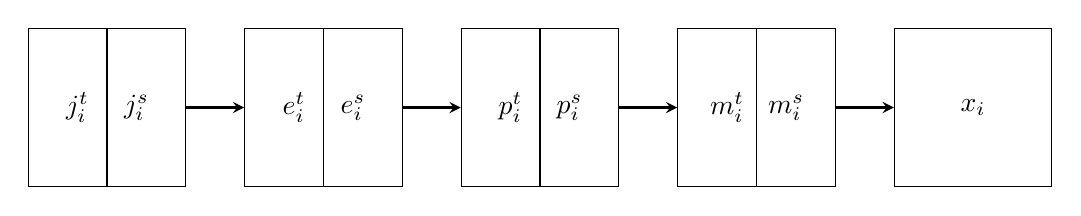
\begin{tikzpicture}
        % Styles for the squares and arrows
        \tikzset{
            square/.style={
                draw,
                rectangle,
                minimum size= 2cm,
                fill=none,
                align=center
            },
            arrow/.style={
                thick,
                ->,
                >=stealth 
            }
        } 
        % Define initial position and shift for squares
        \def\initpos{0}
        \def\shift{2.75}  % Distance between centers of squares
        % Custom labels for each step in the process
        \def\labelsT{{"j_i^t", "e_i^t", "p_i^t", "m_i^t"}}
        \def\labelsS{{"j_i^s", "e_i^s", "p_i^s", "m_i^s"}}
        % Drawing the squares, split squares, and arrows
        \foreach \i in {0,...,4} {
            % Draw split square for the first four
            \ifnum\i<4
                \node[square] (square\i) at (\initpos+\shift*\i,0) {};
                \draw (square\i.south) -- (square\i.north);
                \node at ([xshift=-0.375cm] square\i.center) {$\pgfmathparse{\labelsT[\i]}\pgfmathresult$};
                \node at ([xshift=0.375cm] square\i.center) {$\pgfmathparse{\labelsS[\i]}\pgfmathresult$};
            \else
                % Draw the unsplit square for the fifth one
                \node[square] (square\i) at (\initpos+\shift*\i,0) {$x_i$};
            \fi
            % Draw arrow to next square
            \ifnum\i>0
                \draw[arrow] (square\the\numexpr\i-1\relax.east) -- (square\i.west);
            \fi
        }
    \end{tikzpicture}
    
    \vspace{1em}
    
    \begin{center}
        \small
        \begin{tabular}{lll}
            \textbf{Notation} & \textbf{Description} & \textbf{Dimensions} \\
            \hline
            $j_i^{t/s}$ & Split to task and skill components of $j_i$ & text \\
            $e_i^{t/s}$ & $\text{SBERT}(j_i^{t/s})$ & $384 \times 1$ \\
            $p_i^{t/s}$ & $\text{PCA}(e_i^{t/s})$  & $124 \times 1$ (tasks), $49 \times 1$ (skills) \\
            $m_i^{t/s}$ & $\text{FuzzyC}(p_i^{t/s})$  & $k_t \times 1$ , $k_s \times 1$  \\
            $x_i$ & $m_i^t \oplus m_i^s$ & $k_t + k_s \times 1$ \\
        \end{tabular}
    \end{center}
    
    \caption{This is a pictorial representation of the vectorization process that captures the information in a job posting to a numerical vector. The table provides a summary of the notation and dimensions used at each step of the process.}
    \label{fig:job-vectorization}
\end{figure}


\subsection{Distance Metric Learning}

Having established a numerical representation of job descriptions through our two-stage dimension reduction, 
we now focus on calibrating a distance metric to effectively capture meaningful differences between positions. 
Our approach combines the rich representations derived from pre-trained language models with historical selection 
decisions as a supervisory signal. These past decisions serve as ground truth, helping us identify which aspects 
of job posting content are truly informative for predicting successful hires. Importantly, we do not inject 
selection outcome information into the job postings themselves; rather, historical data guides our metric 
to emphasize the inherently predictive differences in posting content.

Learning a custom metric offers significant advantages over generic distance measures in assessing job posting 
informativeness. Traditional metrics like Euclidean distance treat all dimensions equally, failing to capture 
the varying importance of different skills and responsibilities in actual hiring decisions. Through metric 
learning, we calibrate the weights of our representation vector $(x_i)$ based on how informatively different 
aspects of posting content differentiated between successful and unsuccessful applications. Consider a 
software development position requiring both core technical skills (e.g., expertise in Mainframe development) 
and general workplace skills (e.g., presentation software proficiency). Our metric learns to emphasize 
substantial differences in core technical requirements, which historically strongly predicted selection outcomes, 
while de-emphasizing variations in general skills that had minimal impact on hiring decisions.

We employ the family of Mahalanobis distances, parameterized by a positive semi-definite matrix $(M)$, where 
dimensions are weighted according to their informativeness in distinguishing successful applications. In the 
diagonal case, where $(M)$ contains only diagonal entries, the distance calculation represents an independent 
scaling of each dimension---stretching those that historically differentiated outcomes and compressing less 
informative ones. When $(M)$ is non-diagonal, it can capture more complex relationships through both scaling 
and rotation of the feature space, revealing subtle but informative patterns in the posting content. Formally, 
we define our distance function as:

\begin{equation}
d(x_v, x_c; M) = \sqrt{(x_v - x_c)^T M (x_v - x_c)}
\end{equation}

where $(x_v)$ represents the vector of the sought vacancy, $(x_c)$ represents the vector of the current job, 
and $(M)$ is our calibrated Mahalanobis matrix.

To calibrate $M$, we utilize a dataset $(A)$ of tuples $((x_v, x_c, S_{v,c}))$, comprising vector representations 
of vacancy and current job descriptions with their corresponding selection outcomes. We employ the Mahalanobis 
Metric for Clustering (MMC) algorithm \citep{Xing2002}, which solves:

\begin{align*}
\text{Maximize:} \quad & \sum_{(v,c): S_{v,c} = 0} d(x_v, x_c; M) \\[1em]
\text{Subject to:} \quad & \sum_{(v,c): S_{v,c} = 1} d(x_v, x_c; M)^2 \leq 1 \\
& M \succeq 0
\end{align*}

This formulation calibrates the metric to distinguish between successful and unsuccessful applications by 
maximizing distances between rejected pairs while maintaining bounded distances for selected pairs. Implementation 
uses Python 3.11 and scikit-learn, leveraging 1,060 observations (75\% of our selection decisions) for training. 
The dimensionality of $(M)$, determined by our FCM clustering parameters, influences the granularity of our 
representation of informative skill and task profiles, which we optimize through parameter tuning as discussed next.


\subsection{Parameter Tuning}

To implement the Mahalanobis Metric for Clustering (MMC) algorithm effectively, we need to determine the
optimal number of clusters for the Fuzzy C-Means (FCM) step: $(k_t)$ for task embeddings and $(k_s)$ for skill
embeddings. These parameters directly determine how finely our representation can distinguish between
different types of job postings. The choice of cluster numbers influences our ability to capture meaningful
distinctions between positions while avoiding overly granular distinctions that might not generalize well.
Selecting appropriate values is crucial for creating a representation that effectively captures the
underlying patterns in our hiring data and leads to the most accurate distance metric for predicting
selection probabilities.

Utilizing our dataset of 1,370 internal applications and their outcomes (excluding cases where internal
candidates were rejected in favor of other internal applicants), we employ a rigorous 5-fold cross-validation
strategy on the application dataset $(A)$. For each fold, we test combinations of $(k_s)$ and $(k_t)$, where
$k_s, k_t \in \{2, 3, \ldots, 20\}$, subject to the constraint $k_s + k_t < 25$. This constraint serves a
practical purpose: with limited training data, allowing the dimensionality of the Mahalanobis matrix $(M)$
to grow too large risks overfitting and poor generalization. For each combination, we train the MMC algorithm
on the reduced-dimensional representations derived from the SBERT embeddings and FCM, evaluating performance
on the held-out fold using the Area Under the Receiver Operating Characteristic Curve (AUC).

Our cross-validation analysis, visualized in Figure \ref{fig:AUC}, reveals that optimal performance
is achieved with $k_s = 17$ skill clusters and $k_t = 3$ task clusters, yielding an average AUC of 0.62.
This substantial imbalance between the number of skill and task clusters---17 versus 3---aligns with our intuition
about job postings: while technical skills tend to be numerous and specific (e.g., programming languages,
tools, frameworks), job tasks often fall into broader categories (e.g., development, maintenance, management).
The data-driven optimization of these parameters ensures our representation captures meaningful patterns while
maintaining generalizability.

\begin{figure}[htb]
\centering
\includegraphics[width=0.75\textwidth]{new_img/chart.png}
\caption{Cross-validated AUC scores across different total dimensionalities ($k$), showing optimal performance at $k = 20$}
\label{fig:AUC}
\end{figure}

\subsection{Value of Learning a Custom Distance Metric}

To demonstrate the advantages of learning a distance metric tailored to our organization's selection process, 
we compare our approach against a strong baseline: the cosine distance calculated directly on Sentence-BERT 
embeddings. This comparison helps quantify the value added by our custom metric learning process.

\textbf{SBERT Cosine Distance Baseline:} We established our baseline using the cosine similarity between 
384-dimensional Sentence-BERT embeddings of vacancy and applicant job descriptions. For this baseline, 
we used the 'no-split' approach, concatenating the 'Mandatory Skills,' 'Desired Skills,' and 'Responsibilities' 
sections before embedding. The resulting cosine similarity scores range from -1 to 1, with higher values 
indicating greater semantic overlap between positions. While this approach effectively captures general 
semantic relationships between texts, it treats all aspects of similarity equally, without accounting for 
which differences are most predictive of selection decisions in our specific context.

\textbf{Comparative Analysis:} We evaluated both approaches—the SBERT cosine distance baseline and our 
learned Mahalanobis distance—using the Area Under the Receiver Operating Characteristic Curve (AUC). 
The baseline achieved an AUC of 0.562, indicating some predictive power even with a general semantic 
similarity measure. Our full pipeline, incorporating separate skill and task embeddings with optimal 
cluster parameters ((k_s = 17), (k_t = 3)), achieved a substantially higher AUC of 0.62.

\textbf{Significance of Improvement:} The improvement in AUC from 0.562 (SBERT cosine distance) to 0.62 
(learned Mahalanobis distance) demonstrates the value of our metric learning approach. This gain reflects 
our metric's ability to capture organization-specific patterns in hiring decisions that go beyond general 
semantic similarity. The learned Mahalanobis distance has adapted to recognize which aspects of 
job descriptions are truly predictive of successful hires within our organization. This tailored approach 
leads to more accurate assessments of job fit, with the AUC of 0.62 indicating that our method will 
correctly rank a randomly chosen selected applicant above a randomly chosen rejected applicant 
62\% of the time—a meaningful improvement over both chance (50\%) and the baseline (56.2\%). 
This improvement validates our core premise that job posting text contains valuable information 
about position requirements that can be extracted through careful methodology.